\section{Distribución normal}

La distribución normal es la distribución continua más importante en estadística
y aparece en el \emph{Teorema del Límite Central}.

\begin{definicion}[Distribución normal]
Una variable aleatoria continua $X$ tiene \emph{distribución normal} con parámetros
$\mu$ (media) y $\sigma > 0$ (desviación estándar) si su función de densidad es
\begin{align}
 \label{eq:2.8.3}
 f(x) = \frac{1}{\sigma\sqrt{2\pi}}\,\exp\!\left(-\frac{(x-\mu)^2}{2\sigma^2}\right),
 \qquad x \in \mathbb{R}.
\end{align}
Escribimos $X \sim N(\mu, \sigma^2)$.
\end{definicion}

{Propiedades de la distribución normal} Si $X \sim N(\mu,\sigma^2)$, entonces
\begin{itemize}
 \item La distribución es \emph{simétrica} respecto a $\mu$.
 \item $\mu$ es la media, mediana y moda.
 \item $\sigma^2$ es la varianza.
 \item Si $Z \sim N(0,1)$ (forma estándar), entonces
 $X = \mu + \sigma Z$.
\end{itemize}

{Forma estándar} Si $X \sim N(\mu, \sigma^2)$, la variable estandarizada
\begin{align}
 \label{eq:2.8.4}
 Z = \frac{X - \mu}{\sigma}
\end{align}
sigue una distribución $N(0,1)$ con densidad
\begin{align}
 \label{eq:2.8.5}
 \varphi(z) = \frac{1}{\sqrt{2\pi}}\,e^{-z^2/2}, \qquad z \in \mathbb{R}.
\end{align}

{Regla empírica $68$--$95$--$99.7$} Si $X \sim N(\mu,\sigma^2)$, entonces
\begin{align}
 P(\mu - \sigma \leq X \leq \mu + \sigma) &\approx 0.6827, \\
 P(\mu - 2\sigma \leq X \leq \mu + 2\sigma) &\approx 0.9545, \\
 P(\mu - 3\sigma \leq X \leq \mu + 3\sigma) &\approx 0.9973.
\end{align}

\begin{observacion}
La distribución normal aparece en muchas situaciones prácticas: errores de medición,
altura de personas, puntajes de exámenes, etc. Además, por el Teorema del Límite
Central, la suma (o promedio) de muchas variables aleatorias independientes (bajo
condiciones suaves) se aproxima a una normal.
\end{observacion}

\begin{ejemplo}
 \label{exmp:2.8.2}
Las calificaciones de un examen siguen una distribución $N(70, 100)$ (media $70$,
varianza $100$, es decir, $\sigma=10$). ¿Qué porcentaje de estudiantes obtuvo entre
$60$ y $80$ puntos?
\end{ejemplo}

\begin{solucion}
Estandarizamos: si $X \sim N(70, 100)$, entonces
\begin{align}
 P(60 \leq X \leq 80) = P\!\left(\frac{60-70}{10} \leq Z \leq \frac{80-70}{10}\right)
 = P(-1 \leq Z \leq 1).
\end{align}

Por la regla empírica, este valor es aproximadamente $0.6827 = 68.27\%$.
Usando tablas o software, el valor exacto es $\Phi(1) - \Phi(-1) = 0.8413 - 0.1587 = 0.6827$.
\end{solucion}

\lstinputlisting[language=Python]{../code/distribuciones-continuas-avanzadas/distNormalContinua.py}

\begin{figure}
 \centering
 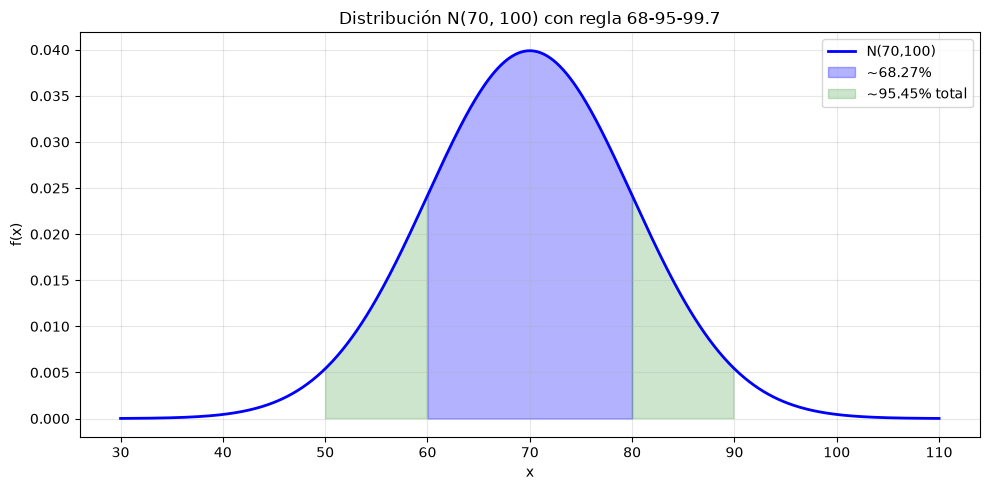
\includegraphics[height=7cm,keepaspectratio=true]{./pe/distNormalContinua.png}
 % distNormalContinua.png: 0x0 pixel, 300dpi, 0.00x0.00 cm, bb=
 \caption{Distribución $N(70,100)$ mostrando la regla empírica 68--95--99.7.}
 \label{fig:2.8.2}
\end{figure}


